\clearpage
\phantomsection

\setcounter{chapter}{0}
\chapter[MÔ HÌNH KÊNH VÀ CÁC PHƯƠNG PHÁP NHẬN DẠNG HỆ THỐNG TRONG MIMO KÍCH THƯỚC LỚN]{Mô hình kênh và các phương pháp nhận dạng hệ thống trong MIMO kích thước lớn}
\label{sec:back}
Việc nhận dạng hệ thống trong truyền thông không dây đã luôn được phát triển ngay từ những thế hệ mạng không dây như 2G~\cite{Tse2005}. Bước đầu tiên trong bài toán nhận dạng là đo đạc và mô hình hoá kênh truyền vô tuyến dưới các dạng biểu diễn toán học khác nhau. Trong phần đầu tiên của chương này, tác giả sẽ trình bày khái quát về một số phương pháp mô hình kênh truyền xác định và ngẫu nhiên khác nhau để chọn ra phương pháp mô hình hoá kênh truyền phù hợp sử dụng trọng luận văn. Tiếp đó, các phương pháp nhận dạng hệ thống MIMO kích thước lớn được phân loại thành 4 hướng tiếp cận và khảo sát một cách khái quát, để chỉ ra các phương pháp ``tri thức mới'' mà luận văn quan tâm.

\section{Mô hình kênh trong hệ thống MIMO kích thước lớn}

\begin{figure}[H]
    \centering
    \begin{tikzpicture}
        \node (b21) [process, align=center, fill=red!10!white] at (0mm, 0mm) {Mô hình kênh xác định};

        \node (b22) [process, align=center, fill=red!10!white] at (70mm, 0mm) {Mô hình kênh ngẫu nhiên};

        \node (b31) [process, align=left, fill=green!10!white] at (-17mm, -20mm) {Đo đạc};

        \node (b32) [right=5mm of b31, process, align=left, fill=green!10!white] {Phân tích theo tia};

        \node (b33) [process, align=left, fill=green!10!white] at (53mm, -20mm) {CBSM};

        \node (b34) [right=5mm of b33, process, align=left, fill=green!10!white] {GBSM};

        \draw[arrow] (b21) -- (b31);
        \draw[arrow] (b21) -- (b32);
        \draw[arrow] (b22) -- (b33);
        \draw[arrow] (b22) -- (b34);
        
    \end{tikzpicture}
    \caption{Phân loại mô hình kênh truyền xác định và ngẫu nhiên trong MIMO kích thước lớn.}
    \label{fig:classify_MIMO}
\end{figure}

Trong các hệ thống mMIMO, công bố~\cite{Feng2022} đã khảo sát các mô hình kênh truyền tiên tiến và phân loại chúng theo các hướng tiếp cận khác nhau. Từ đó, trong luận văn này, các mô hình kênh truyền trong hệ mMIMO được xem xét chia thành hai kiểu chính là mô hình kênh truyền xác định và mô hình kênh truyền ngẫu nhiên. Các mô hình kênh truyền xác định có thể chia thành hai loại nhỏ hơn là phương pháp đo đạc và kỹ thuật phân tích theo tia. Với mô hình kênh truyền ngẫu nhiên, hai kiểu chính đó là mô hình ngẫu nhiên dựa trên tương quan (CBSM - Correlation-based stochastic model) và mô hình ngẫu nhiên dựa trên hình học (GBSM - Geometry-based stochastic model).

\subsection{Mô hình kênh truyền xác định}

\begin{figure}[ht]
    \centering
    \begin{tikzpicture}
        \node[antenna, thick, scale=0.6] at (0, 0) (Tx0) {};
        \node at (0, 17mm) (text_Tx0) {Tx $0$};
        \draw[line] (-10mm, 0) -- (Tx0) node [pos=0, left] {$\mathbf{s}_0$};

        \node[antenna, thick, scale=0.6] at (0, -25mm) (Tx1) {};
        \node at (0, -8mm) (text_Tx1) {Tx $1$};
        \draw[line] (-10mm, -25mm) -- (Tx1) node [pos=0, left] {$\mathbf{s}_1$};

        \node[scale=1.5] at (0, -30mm) (dotss) {$\mathbf{\vdots}$};

        \node[antenna, thick, scale=0.6] at (0, -55mm) (TxT) {};
        \node at (0, -38mm) (text_TxT) {Tx $T-1$};
        \draw[line] (-10mm, -55mm) -- (TxT) node [pos=0, left] {$\mathbf{s}_{T-1}$};

        \node[antenna, thick, scale=0.6] at (70mm, 0) (Rx0) {};
        \node at (70mm, 17mm) (text_Rx0) {Rx $0$};
        \draw[line] (80mm, 0) -- (Rx0) node [pos=0, right] {$\mathbf{x}_{0}$};

        \node[antenna, thick, scale=0.6] at (70mm, -25mm) (Rx1) {};
        \node at (70mm, -8mm) (text_Rx1) {Rx $1$};
        \draw[line] (80mm, -25mm) -- (Rx1) node [pos=0, right] {$\mathbf{x}_{1}$};

        \node[scale=1.5] at (70mm, -30mm) (dotss) {$\mathbf{\vdots}$};

        \node[antenna, thick, scale=0.6] at (70mm, -55mm) (RxL) {};
        \node at (70mm, -38mm) (text_RxL) {Rx $L - 1$};
        \draw[line] (80mm, -55mm) -- (RxL) node [pos=0, right] {$\mathbf{x}_{L-1}$};

        \draw[arrow] (3mm, 6mm) -- (67mm, 6mm);
        \draw[arrow] (3mm, 5mm) -- (67mm, -20mm);
        \draw[arrow] (3mm, 4mm) -- (67mm, -49mm);

        \draw[arrow] (3mm, -19mm) -- (67mm, 5mm);
        \draw[arrow] (3mm, -20mm) -- (67mm, -21mm);
        \draw[arrow] (3mm, -21mm) -- (67mm, -50mm);

        \draw[arrow] (3mm, -49mm) -- (67mm, 4mm);
        \draw[arrow] (3mm, -50mm) -- (67mm, -22mm);
        \draw[arrow] (3mm, -51mm) -- (67mm, -51mm);

        \node at (35mm, -60mm) (H) {$\mathbf{H} \in \mathbb{C}^{L \times T}$};
    \end{tikzpicture}
    \caption{Mô hình minh hoạ hệ thống truyền thông mMIMO.}
    \label{fig:sys_model}
\end{figure}

Để đi vào chi tiết hơn vào các mô hình kênh kể trên, trước hết, xem xét một mô hình hệ thống thu phát mMIMO đơn giản với $T$ ăng-ten phát và $L$ ăng-ten thu như trên hình~\ref{fig:sys_model}. Có thể minh hoạ hệ thống thu phát dưới dạng toán học, tại thời điểm $n$
\begin{equation}
    \mathbf{x}(n) = \mathbf{H}(n)\mathbf{s}(n) + \mathbf{w}
\end{equation}
trong đó $\mathbf{s}(n) \in \mathbb{C}^{T \times 1}$ là các ký hiệu được gửi đi từ $T$ bộ phát. Kênh truyền được biểu diễn là ma trận $\mathbf{H} \in \mathbb{C}^{L\times T}$. Tiếp đến, $\mathbf{x}(n) \in \mathbb{C}^{L \times 1}$ là véc-tơ biểu diễn tín hiệu thu được từ $L$ ăng-ten. Cuối cùng, $\mathbf{w} \in \mathbb{C}^{L \times 1}$ đại diện cho tạp âm trắng cộng sinh (AWGN - Additive white Gaussian noise). 

\subsubsection{Mô hình kênh truyền xác định dựa trên máy đo}

Mô hình kênh truyền dựa trên đo đạc là phương pháp mô hình hoá kênh truyền tiệm cận với kênh truyền vô tuyến thực. Phương pháp mô hình kênh này mang tính thực nghiệm, trong các điều kiện cụ thể, như môi trường trong nhà~\cite{Li2018, Willhammar2020}, khu ngoại ô~\cite{Hao2019}, sân vận động~\cite{Liu2015},~\ldots. Việc đo đạc của các công bố kể trên thường dựa trên các thiết lập cụ thể, sử dụng các thiết bị chuyên dụng như máy phân tích mạng và các bộ phát sóng tiêu chuẩn. Trên bảng~\ref{tab:measurement} là danh sách của 5 nghiên cứu kênh truyền thực tế dựa trên đo đạc. Có thể nhận thấy rằng, các mô hình này có những thông số rất riêng biệt như tần số hoạt động, băng thông, hay trong một môi trường cố định biết trước. Ngoài ra, trong mỗi công bố, các thông số đo được từ máy phân tích chuẩn chỉ phản ánh một số tính chất (DoA, DoD, số cụm, phân cực chéo,~\ldots) của kênh truyền vô tuyến. Từ các thông số này, sử dụng giải thuật SEGA~\cite{Fleury1999} để khôi phục lại các hệ số của kênh truyền một cách chính xác.

\begin{table}[ht]
\centering
\caption{Các mô đặc trưng kênh truyền mMIMO dựa trên đo đạc~\cite{Feng2022}.}
\label{tab:measurement}
\resizebox{\textwidth}{!}{%
\begin{tabular}{|l|l|l|l|l|l|} 
\hline
\multicolumn{1}{|c|}{\vcell{\textbf{Công bố}}} & \multicolumn{1}{c|}{\vcell{\textbf{Tần số}}} & \multicolumn{1}{c|}{\vcell{\textbf{Băng thông}}} & \multicolumn{1}{c|}{\vcell{\textbf{Môi trường truyền}}} & \multicolumn{1}{c|}{\vcell{\begin{tabular}[b]{@{}c@{}}\textbf{Cấu hình mảng}\\\textbf{ăng-ten ($T \times L$)}\end{tabular}}} & \multicolumn{1}{c|}{\vcell{\textbf{Thông số đo đạc}}} \\[-\rowheight]
\multicolumn{1}{|c|}{\printcelltop} & \multicolumn{1}{c|}{\printcelltop} & \multicolumn{1}{c|}{\printcelltop} & \multicolumn{1}{c|}{\printcelltop} & \multicolumn{1}{c|}{\printcelltop} & \multicolumn{1}{c|}{\printcelltop} \\ 
\hline
\vcell{\cite{Li2018}} & \vcell{11 GHz} & \vcell{200 MHz} & \vcell{Rạp chiếu phim} & \vcell{1 $\times$ 256} & \vcell{\begin{tabular}[b]{@{}l@{}}Phân cực chéo,\\Góc phát (DoD)\end{tabular}} \\[-\rowheight]
\printcelltop & \printcelltop & \printcelltop & \printcelltop & \printcelltop & \printcelltop \\ 
\hline
\vcell{\cite{Willhammar2020}} & \vcell{2,6 GHz} & \vcell{40 MHz} & \vcell{\begin{tabular}[b]{@{}l@{}}Trong nhà,\\Ngoài trời\end{tabular}} & \vcell{1 $\times$ 128} & \vcell{Hệ số khuếch đại} \\[-\rowheight]
\printcelltop & \printcelltop & \printcelltop & \printcelltop & \printcelltop & \printcelltop \\ 
\hline
\vcell{\cite{Hao2019}} & \vcell{3,5 GHz} & \vcell{160 MHz} & \vcell{Khu ngoại ô} & \vcell{32 $\times$ 32} & \vcell{\begin{tabular}[b]{@{}l@{}}PDP - thống kê công suất,\\theo độ trễ, Hệ số $K$,\\Trễ trải\end{tabular}} \\[-\rowheight]
\printcelltop & \printcelltop & \printcelltop & \printcelltop & \printcelltop & \printcelltop \\ 
\hline
\vcell{\cite{Wang2017}} & \vcell{3,5 GHz} & \vcell{200 MHz} & \vcell{\begin{tabular}[b]{@{}l@{}}Khu dân cư~\\kích cỡ macro\end{tabular}} & \vcell{16 $\times$ 256} & \vcell{\begin{tabular}[b]{@{}l@{}}DoA, DoD, \\Số lượng các cụm (TC),\\Vùng hiển thị (VR)\end{tabular}} \\[-\rowheight]
\printcelltop & \printcelltop & \printcelltop & \printcelltop & \printcelltop & \printcelltop \\ 
\hline
\vcell{\cite{Liu2015}} & \vcell{\begin{tabular}[b]{@{}l@{}}1,4725 GHz\\4,45 GHz\end{tabular}} & \vcell{\begin{tabular}[b]{@{}l@{}}91 MHz,\\100 MHz\end{tabular}} & \vcell{Sân vận động} & \vcell{1 $\times$ 128} & \vcell{\begin{tabular}[b]{@{}l@{}}Hệ số kênh truyền,\\Hệ số $K$ của Ricean,\\Trễ trải\end{tabular}} \\[-\rowheight]
\printcelltop & \printcelltop & \printcelltop & \printcelltop & \printcelltop & \printcelltop \\
\hline
\end{tabular}
}
\end{table}

Giải thuật SAGE, viết tắt của Space Alternating Generalized Expectation Maximization, là một giải thuật lặp được sử dụng phổ biến để ước lượng kênh trong hệ thống truyền thông không dây. Phương pháp này lặp lại các bước ước lượng tham số kênh truyền bằng bộ ước lượng hợp lẽ cực đại (MLE - Maximum likelihood estimator) của tín hiệu nhận được dựa trên các tham số ước lượng và thông số từ đo đạc. Một vài bước tổng quan trong giải thuật SAGE như sau
\begin{enumerate}
    \item Khởi tạo ước lượng tham số kênh ban đầu ($\hat{\mathbf{H}}$). Điều này có thể được thực hiện ngẫu nhiên hoặc dựa trên kiến thức trước đó, tùy thuộc vào thông tin có sẵn ($\boldsymbol{\Theta}$).
    \item Với các ước lượng tham số kênh hiện tại, tính kỳ vọng có điều kiện của tín hiệu truyền tải dựa trên tín hiệu nhận được.
    \begin{equation*}
        \hat{\mathbf{s}}_{\hat{\mathbf{H}}} (\boldsymbol{\Theta}) = \mathbb{E} (\mathbf{s} | \mathbf{x}, \boldsymbol\Theta)
    \end{equation*}
    \item Cập nhật ước lượng tham số kênh bằng cách tối đa hóa khả năng của tín hiệu nhận được dựa trên kỳ vọng có điều kiện tính toán ở bước trước đó.
    \begin{equation*}
        \hat{\mathbf{H}} = \min_{\hat{\mathbf{H}}} \hat{\mathbf{s}}_{\hat{\mathbf{H}}} (\boldsymbol{\Theta})
    \end{equation*}
    \item Lặp lại các bước 2 và 3 cho đến khi các ước lượng tham số kênh hội tụ. Sự hội tụ thường được xác định bằng cách theo dõi một tiêu chí hội tụ, chẳng hạn như sự thay đổi trong ước lượng tham số giữa các lần lặp (hàm mất mát).
    \item Sau khi đạt được sự hội tụ, thu được các ước lượng cuối cùng của các tham số kênh.
\end{enumerate}

\subsubsection{Kỹ thuật phân tích theo tia}
Những năm gần đây, một loại mô hình xác định mới được đề xuất cho ra kết quả không thua kém quá nhiều so với việc sử dụng các máy đo chuyên dụng như đã trình bày ở trên, đó là phương pháp phân tích theo tia (RT - Ray-tracing)~\cite{Liu2020}. Dựa trên lợi thế của các mô hình 3D và kỹ thuật RT trong các lĩnh vực khác như trò chơi trực tuyến, nhiều đề xuất sử dụng RT cho mô hình kênh mMIMO với việc coi các đường truyền  vô tuyến giống như các tia sáng lan truyền trong không gian mô phỏng. Ưu điểm của phương pháp này đó là không cần phải đo đạc quá nhiều thông số như các mô hình đo truyền thống. Thay vào đó, các thông số được quan tâm chỉ còn vị trí và hướng của bên thu, phát, cùng mô hình 3D chi tiết của môi trường phát. Đây chính là điểm đặc biệt của phương pháp này, khi mô hình 3D chi tiết của khu dân cư, văn phòng, cần được xây dựng chính xác và chi tiết để làm đầu vào cho RT. Quá trình ray-tracing trong mô hình kênh RT bao gồm các bước sau
\begin{enumerate}
    \item Xác định vị trí và hướng di chuyển của các ăng-ten truyền và nhận trong mMIMO.
    \item Xác định môi trường không gian, bao gồm các đối tượng như tòa nhà, cây cối, và địa hình.
    \item Tạo ra các bức xạ ray từ anten truyền và theo dõi chúng khi chúng tương tác với các đối tượng trong môi trường.
    \item Phân tích sự tương tác của các bức xạ ray với môi trường để tính toán sự suy giảm, phản xạ, giao thoa và nhiễu.
    \item Tính toán các thông số truyền thông như tốc độ bít, tỷ lệ lỗi bít và công suất tín hiệu đến ở các ăng-ten nhận.
\end{enumerate}
Một trong các ứng dụng có thể giúp người dùng thử nghiệm mô hình kênh truyền dựa trên phương pháp RT hiện nay là MatLab R2023a~\cite{RT}, tuy nhiên, các mô hình 3D có sẵn hiện tại chỉ là mô hình đường phố từ các nguồn dữ liệu công khai.

\subsection{Mô hình kênh truyền ngẫu nhiên}

Các mô hình kênh truyền ngẫu nhiên dựa trên các đặc trưng mang tính thống kê của kênh vô tuyến trong mMIMO để đưa ra các giả thiết cho ma trận kênh truyền $\mathbf{H}$. Trong đó, CBSM là mô hình kênh được sử dụng phổ biến nhất trong các nghiên cứu nhận dạng kênh truyền lí thuyết do tính đơn giản của nó. Ngược lại, GBSM phân tích kênh truyền theo hướng vật lí, chia nhỏ việc truyền sóng vô tuyến thành các cụm, đường và xem xét ảnh hưởng của từng thành phần riêng lẻ đến ma trận kênh truyền.

\subsubsection{CBSM}

Xét một biểu diễn ma trận kênh truyền ở dạng đơn giản nhất như sau
\begin{equation}
    \label{eq:unstructure}
    \mathbf{H}_{total} = \alpha \mathbf{H} 
\end{equation}
trong đó, $\alpha$ đại diện cho các ảnh hưởng của kênh truyền ở kích thước lớn (large-scale fading) gồm suy hao (path loss), shadowing như được biểu diễn trên phương trình~(\ref{eq:FSPL}). Ma trận $\mathbf{H}$ đại diện cho ảnh hưởng của kênh truyền ở kích thước nhỏ (small-scale fading), thông thường được biểu diễn dưới dạng ma trận
\begin{equation}
    \mathbf{H} = \begin{bmatrix}
    h_{0,0} & \ldots  & h_{0, T-1} \\ 
    \vdots & \ddots & \vdots\\ 
    h_{L-1, 0} & \ldots  & h_{L-1, T-1}
    \end{bmatrix}
\end{equation}
với mỗi phần tử thứ ($l, t$) tương ứng với đáp ứng xung của kênh giữa ăng-ten phát thứ $t$ và ăng-ten nhận thứ $l$. Điều tương tự với các mô hình băng rộng gồm các độ trễ kênh khác nhau~\cite{Saleh1987}. Nếu các hệ số trong ma trận kênh truyền được giả sử là có phân bố Gaussian phức, ma trận $\mathbf{H}$ có thể được xác định chỉ từ ma trận hiệp phương sai như sau
\begin{equation}
    \label{eq:correlation}
    \operatorname{vec}(\mathbf{H}) = \mathbf{R}^{1/2}_{\text{mMIMO}} \operatorname{vec} (\mathbf{G})
\end{equation}
trong đó, $\operatorname{vec}$ là phép véc-tơ hoá một ma trận, từ $\mathbf{H}$ kích thước $L\times T$ thành $LT \times 1$. $\operatorname{vec}(\mathbf{G})$ là véc-tơ chứa các biến ngẫu nhiên i.i.d Gaussian và phương sai $\sigma$. Ma trận $\mathbf{R}^{1/2}_{\text{mMIMO}}$ mô tả cấu trúc không gian của các mảng mMIMO, trong đó xem xét sự tương quan (correlation) lẫn nhau giữa các phần tử trong ma trận kênh truyền. Ma trận này được ước lượng như sau
\begin{equation}
    \mathbf{R}_{\text{mMIMO}} = \mathbb{E} ({\operatorname{\mathbf{H}} \operatorname{\mathbf{H}}^H})
\end{equation}
với $(.)^H$ là ma trận Hermitian. Trong luận văn này, một trường hoặc đặc biệt của CBSM được xem xét đó là mô hình i.i.d Rayleigh. Mô hình này giả sử không có sự tương quan/ảnh hưởng lẫn nhau giữa các ăng-ten truyền/nhận. Điều này chỉ có được khi số lượng thành phần đa đường nhiều và phân bố đều trong miền không gian. Với giả thiết này, các giá trị trong ma trận tương quan của mMIMO ($\mathbf{R}_{\text{mMIMO}}$) chỉ tương ứng với một giá trị thực duy nhất. Do đó, theo phương trình~(\ref{eq:correlation}), các hệ số trong ma trận $\mathbf{H}$ sẽ là các biến ngẫu nhiên i.i.d Gaussian. Để đơn giản hoá hơn nữa, trong phương trình~(\ref{eq:unstructure}), các ảnh hưởng của kênh truyền ở kích thước lớn ($\alpha$) được gộp vào ma trận $\mathbf{H}$ thành các biến i.i.d Gaussian duy nhất. Trong phần sau của luận văn, mô hình kênh truyền này được gọi là ``\textbf{phi cấu trúc}'' (unstructured) do các ảnh hưởng của kênh đường minh hoạ qua các hệ số kênh duy nhất, không xét đến sự lan truyền của sóng vô tuyến như trong mô hình kênh ``có cấu trúc'' sẽ được trình bày ở mục~\ref{sec:GBSM}.

\subsubsection{GBSM}
\label{sec:GBSM}

GBSM là mô hình kênh có độ phức tạp cao, khi xem xét sự lan truyền của sóng vô tuyến trong không gian dưới dạng các cụm, tia, đường truyền riêng biệt. Đây cũng là phương pháp được sử dụng phổ biến trong các chuẩn truyền thông di động, ví dụ như: 3GPP phiên bản 16~\cite{r16} cho 5G hay WINNER~\cite{WINNER}. Phương pháp mô hình hoá kênh trong các tiêu chuẩn này được chia vào nhánh bán GBSM (semi-GBSM), do vừa dựa trên các thông số ngẫu nhiên và các thông số cố định thu được do đo lường. Như nêu trên, tuy có tính chính xác cao, nhưng do hạn chế về độ phức tạp, nên một phương pháp mô hình kênh GBSM khác chỉ gồm các thành phần ngẫu nhiên có tên ``có cấu trúc'' hay tham số (parametric) cũng sẽ được trình bày ở phần sau.

\begin{figure}
    \centering
    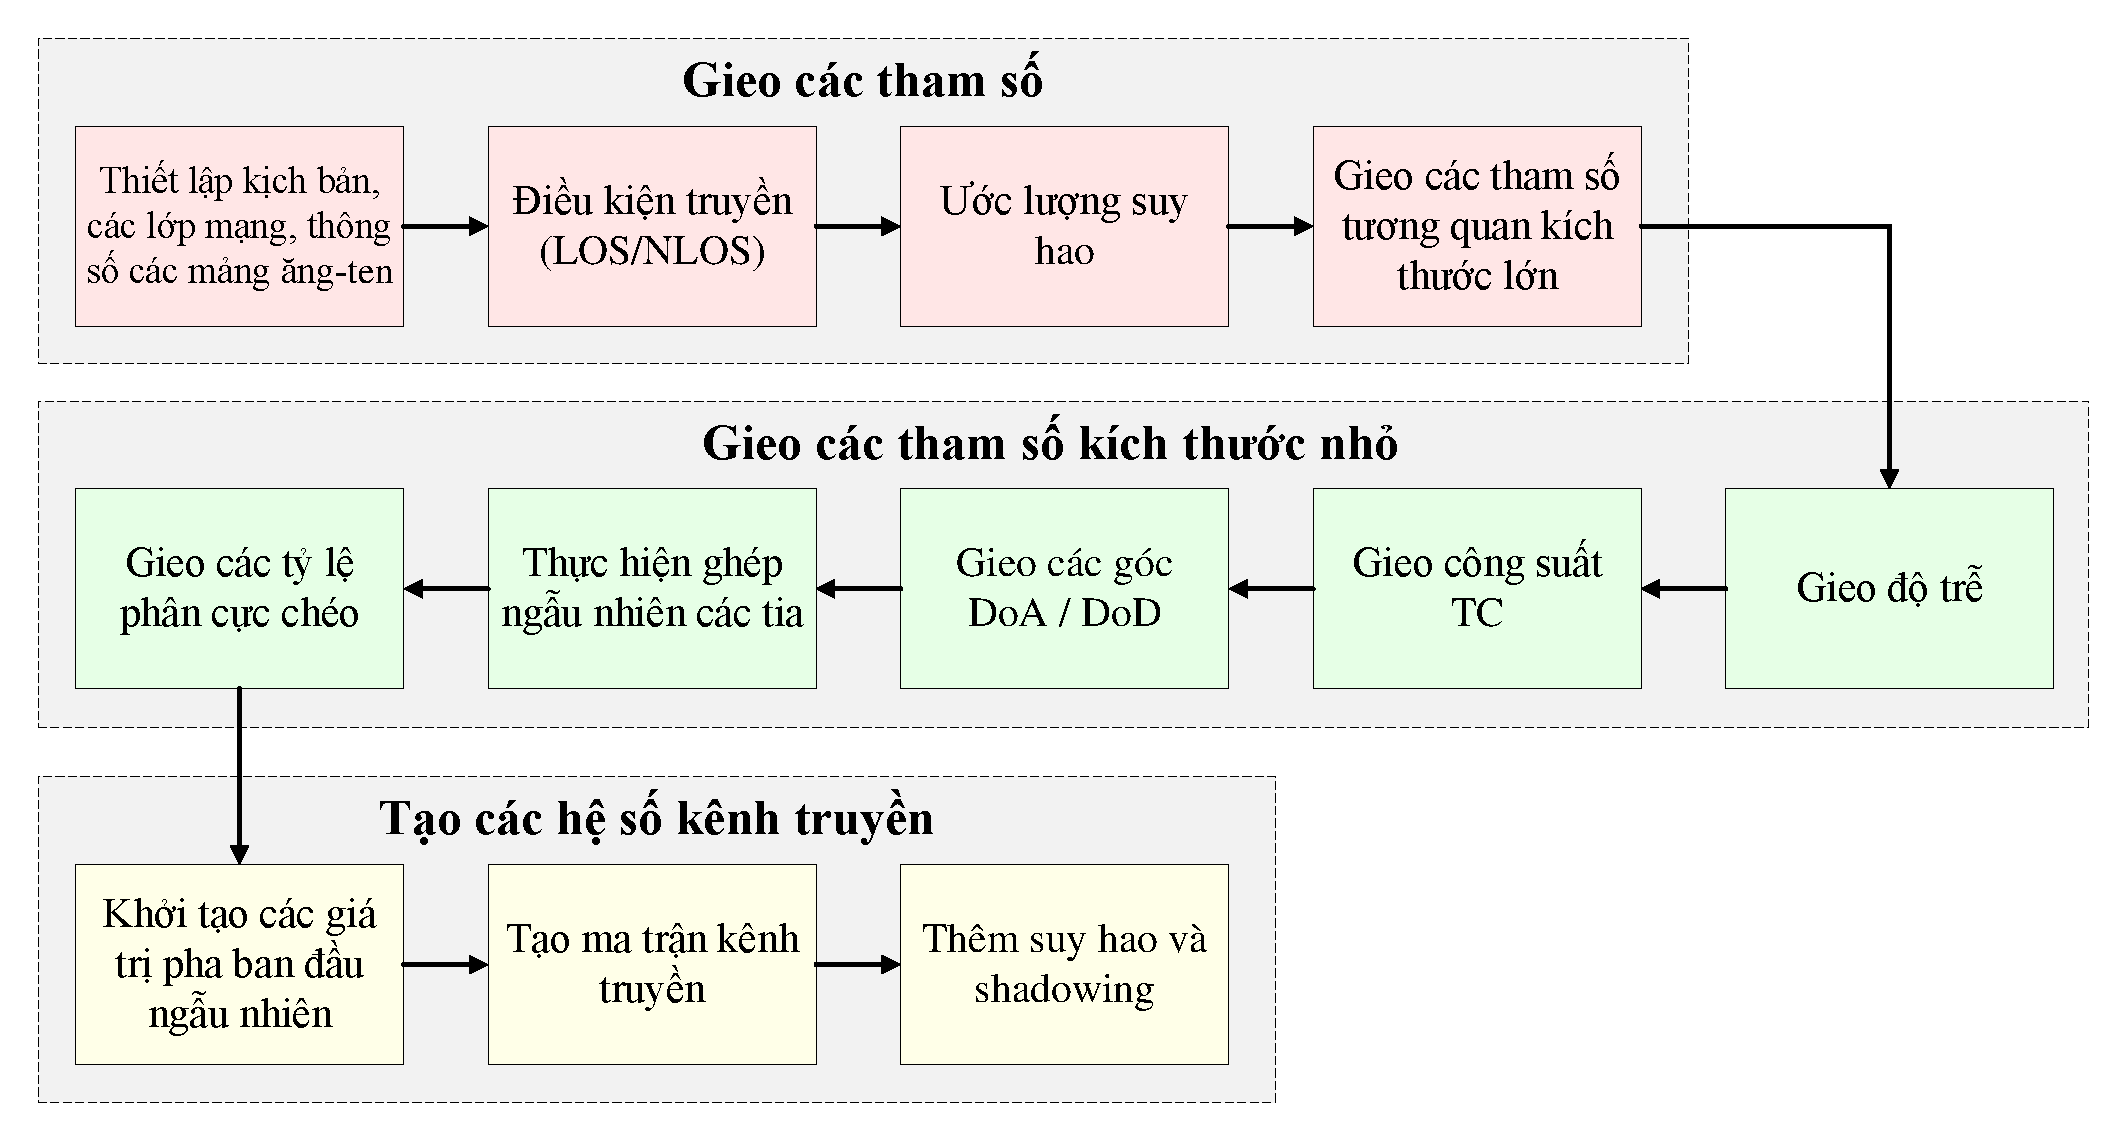
\includegraphics[width=\linewidth]{figures/3GPP_flow.pdf}
    \caption{Các bước tạo mô hình kênh truyền trong tiêu chuẩn 3GPP phiên bản 16~\cite{r16}.}
    \label{fig:3gpp_flow}
\end{figure}

Trên hình~\ref{fig:3gpp_flow} là 12 bước trong quá trình mô hình hoá kênh truyền mMIMO được đề ra trong tiêu chuẩn 3GPP phiên bản 16 dành cho các hệ thống 5G. Phần tiếp theo sẽ trình bày sơ lược về các nét chính trong phương pháp mô hình hoá này. Dạng biểu diễn điển hình của phương pháp mô hình kênh truyền đo đạc như sau~\cite{Ju2021}
\begin{equation}
    \label{eq:3gpp}
    \begin{aligned}
        {h}_{l, t} = \sum\limits_{n=1}^{N} \sum\limits_{m=1}^{M_n} \alpha_{n, m, t} & \cdot e^{i\varphi_{n, m, t}} \cdot \operatorname{sinc}\left(l-\tau_{n, m, t}\right) \\
        &\cdot e^{-i k_d s_t(\theta^d_{n, m, t}, \phi^d_{n, m, t})} e^{-i k_a s_l(\theta^a_{n, m, t}, \phi^a_{n, m, t})} 
    \end{aligned}
\end{equation}
với $l= 0,1,\ldots, L-1$. $N, M_n$ lần lượt là số lượng các cụm phân chia theo thời gian (TC - Time cluster) đến bên thu và số lượng các đường nhỏ hơn (sub-path) trong mỗi cụm kể trên. Với sub-path thứ $m$ trong cụm thứ $n$, $\alpha, \varphi, \tau$ đại diện cho biên độ, pha của sub-path, và thời gian trễ tuyệt đối. Góc ngẩng (zenith) và góc phương vị (azimuth) của hướng sóng đi (DoD - Direction of departure) và hướng sóng đến (DoA) lần lượt là  $\theta^d, \phi^d, \theta^a$, $\phi^a$. Ký hiệu $(\cdot)$ tương ứng là phép nhân vô hướng. Các thành phần biên độ $\alpha_{n,m,t}$ của $\boldsymbol{h}_{l, t}$ lại phụ thuộc vào suy hao, như một hàm của tần số sóng mang ($f_c$), khoảng cách ($d$), cho bởi
\begin{equation}
    \label{eq:FSPL}
    \begin{aligned}
        \alpha_{n, m, t}(f_c, d)[\mathrm{dB}]=& \mathrm{FSPL}\left(f_c, d_{0}\right)+10 n \log _{10}\left(\frac{d}{d_{0}}\right)+\chi_{\sigma}, \\
        & \text { với } d \geq d_{0}, \text { khi } d_{0}=1\mathrm{m}
    \end{aligned}
\end{equation}
trong đó, $\operatorname{FSPL}\left(f_c, d_{0}\right)=20 \log _{10}\left(4 \pi d_{0} c / f_c\right)$, với $c$ là vận tốc ánh sáng, $n$ đại diện cho hệ số mất mát hàm mũ (PLE - Path loss exponent), và $\chi_{\sigma}$ là thành phần shadow fading được mô hình hoá dưới dạng một biến ngẫu nhiên lognormal với trung bình không và độ lệch chuẩn $\sigma$. Các thông số trong các phương trình (\ref{eq:3gpp}) và (\ref{eq:FSPL}) được quy định và đo đạc xác định cho từng môi trường khác nhau. Đầu tiên, cần xác định số lượng các TC trong một môi trường cụ thể, trên bảng~\ref{tab:num_TC} chỉ ra các thông số được đo đạc này cho 4 loại môi trường cụ thể, bao gồm: UMi - khu dân cư kích cỡ micro, UMa - khu dân cư kích cỡ macro, RMa - khu nông thông kích cỡ macro, và điều kiện văn phòng trong nhà. Mỗi môi trường trên, các kịch bản đo được thiết lập ở 2 hoặc 3 tình huống gồm: tầm nhìn thẳng (LOS - Line of sight), không tầm nhìn thẳng (NLOS - non-LOS), và từ bên ngoài vào trong nhà (O2I - Outdoor to indoor).
\begin{table}
\centering
\caption{Số lượng các TC và sub-path trong mỗi TC theo chuẩn 3GPP phiên bản 16~\cite{r16}.}
\label{tab:num_TC}
\begin{tabular}{|l|c|c|c|c|c|c|} 
\hline
\multicolumn{1}{|c|}{\multirow{2}{*}{\textbf{Thông số ~}}} & \multicolumn{3}{c|}{\begin{tabular}[c]{@{}c@{}}\textbf{UMi - Khu dân cư,}\\\textbf{kích cỡ micro}\end{tabular}} & \multicolumn{3}{c|}{\begin{tabular}[c]{@{}c@{}}\textbf{UMa - Khu dân cư,}\\\textbf{~kích cỡ macro~}\end{tabular}} \\ 
\cline{2-7}
\multicolumn{1}{|c|}{} & \textbf{LOS} & \textbf{NLOS} & \textbf{O2I} & \textbf{LOS} & \textbf{NLOS} & \textbf{O2I} \\ 
\hline
\textbf{Số lượng TC} & 12 & 19 & 12 & 12 & 20 & 12 \\ 
\hline
\textbf{Số lượng sub-path mỗi TC} & 20 & 20 & 20 & 20 & 20 & 20 \\ 
\hline
\multirow{2}{*}{\textbf{Thông số}} & \multicolumn{3}{c|}{\begin{tabular}[c]{@{}c@{}}\textbf{\textbf{RMa - Khu nông thôn,}}\\\textbf{\textbf{~kích cỡ macro~}}\end{tabular}} & \multicolumn{3}{c|}{\begin{tabular}[c]{@{}c@{}}\textbf{\textbf{Văn phòng,}}\\\textbf{\textbf{~trong nhà}}\end{tabular}} \\ 
\cline{2-7}
 & \textbf{LOS} & \textbf{NLOS} & \textbf{O2I} & \textbf{LOS} & \multicolumn{2}{c|}{\textbf{NLOS}} \\ 
\hline
\textbf{Số lượng TC} & 11 & 10 & 10 & 15 & \multicolumn{2}{c|}{19} \\ 
\hline
\textbf{Số lượng sub-path mỗi TC} & 20 & 20 & 20 & 20 & \multicolumn{2}{c|}{20} \\
\hline
\end{tabular}
\end{table}

Tiếp đến, độ dịch pha ban đầu của các sub-path trong mỗi TC cũng được 3GPP đưa ra như trên bảng~\ref{tab:phase}.
\begin{table}
\centering
\caption{Độ lệch pha của các sub-path trong một TC.}
\label{tab:phase}
\begin{tabular}{|c|c|c|c|} 
\hline
\multicolumn{1}{|c|}{\textbf{sub-path \#}} & \multicolumn{1}{c|}{$\varphi_{n,m,t} (^\circ)$} & \textbf{\textbf{sub-path \#}} & $\varphi_{n,m,t} (^\circ)$ \\ 
\hline
1, 2 & $\pm$ 0,0447 & 11, 12 & $\pm$0,6797 \\ 
\hline
3, 4 & $\pm$ 0,1413 & 13, 14 & $\pm$0,8844 \\ 
\hline
5, 6 & $\pm$ 0,2492 & 15, 16 & $\pm$1,1481 \\ 
\hline
7, 8 & $\pm$ 0,3715 & 17, 18 & $\pm$1,5195 \\ 
\hline
9, 10 & $\pm$ 0,5129 & 19, 20 & $\pm$2,1551 \\
\hline
\end{tabular}
\end{table}

Thông tin về tỷ lệ công suất của các sub-path trong mỗi TC và độ trễ của chúng so với sub-path đến sớm nhất được trình bày trên bảng~\ref{tab:SC}. Cụ thể, mỗi TC sẽ được chia nhỏ hơn nữa thành 3 cụm con (SC - sub-cluster). Các sub-path sẽ được chia vào một trong ba SC trên dựa trên thời gian trễ của chúng so với tia đến sớm nhất. Bốn thông số còn lại bao gồm $\theta$ và $\phi$ của bên thu và phát lần lượt được biểu diễn dưới dạng các giá trị ngẫu nhiên thuộc các phân bố khác nhau tuỳ thuộc vào điều kiện môi trường, chi tiết xem trong các bảng từ 7.5-6 đến 7.5-10 tại~\cite{r16}.
\begin{table}
\centering
\caption{Thông tin về công suất và độ trễ của các sub-path trong mỗi TC.}
\label{tab:SC}
\begin{tabular}{|c|c|c|c|} 
\hline
\vcell{\textbf{SC \#}} & \vcell{\textbf{sub-path \#}} & \vcell{\begin{tabular}[b]{@{}c@{}}\textbf{Tỷ lệ công suất}\\\textbf{($\alpha_{n, m, t} / \sum_{m=1}^{M} \alpha_{n, m, t}$)}\end{tabular}} & \vcell{\begin{tabular}[b]{@{}c@{}}\textbf{Trễ tuyệt đối}\\\textbf{($\tau_{n, m, t} - \tau_{n, 1, t}$)}\end{tabular}} \\[-\rowheight]
\printcelltop & \printcelltop & \printcelltop & \printcelltop \\ 
\hline
1 & 1, 2, 3, 4, 5, 6, 7, 8, 19, 20 & 10/20 & 0 ns \\ 
\hline
2 & 9, 10, 11, 12, 17, 18 & 6/20 & 5 ns \\ 
\hline
3 & 13, 14, 15, 16 & 4/20 & 10 ns \\
\hline
\end{tabular}
\end{table}

Một phương pháp mô hình hoá kênh truyền GBSM khác, với độ phức tạp nhỏ hơn đó là parametric hay specular~\cite{Le2018, Swindlehurst2022}. Mô hình này vẫn kế thừa đặc trưng không gian của GBSM khi xem xét việc truyền sóng theo các đường khác nhau trong không gian 3D ($\varphi$). Tuy nhiên, thay vì chia thành các cụm, sub-path với các góc, độ trễ khác nhau, specular gộp các cụm (TC) thành các đường truyền lớn do xem xét đặc trưng là tính thưa trong các hệ truyền thông sử dụng sóng mi-li-mét. Các thành phần suy hao, dịch pha, và độ trễ được gộp chung lại thành một hệ số khuếch đại phức ($\beta$).
\begin{equation}
    h_{l, t} = \sum\limits_{n=0}^{N-1} \beta_{n, t} = \sum\limits_{n=0}^{N-1} \beta_{n, t} \cdot e^{\varphi_{l, n, t}} 
\end{equation}
các giá trị $\beta, \varphi(\theta, \phi)$ trong mô hình kể trên thường sẽ được gieo ngẫu nhiên theo các phân bố biết trước. Chi tiết hơn vê mô hình kênh parametric có tại chương~\ref{sec:CRB}. Trong phần sau của luận văn, mô hình kênh truyền này được gọi là ``\textbf{có cấu trúc}'' (structured) để phân biệt với phi cấu trúc trong mục CBSM ở trên.

\subsubsection{Đánh giá các phương pháp mô hình kênh cho mMIMO}

Dựa trên~\cite{Feng2022}, có ba thông số để đánh giá một mô hình kênh truyền bao gồm: tính chính xác (sự tương quan của mô hình và kênh thực), độ phức tạp (lượng tính toán cần để tạo ra một mô hình kênh), và tính tổng quát (mô hình kênh có phù hợp với nhiều kịch bản kênh truyền khác nhau hay không?).

Cũng trong~\cite{Feng2022}, nhóm tác giả đã chỉ ra thông qua mô phỏng, semi-GBSM là phương pháp cho tốc độ bít lớn nhất tương đương với mô hình kênh truyền xác định qua đo đạc, do đây cũng là hai phương pháp gần nhất với môi trường truyền thông không dây thực tế. Điểm hạn chế của cả hai phương pháp xác định và semi-GBSM nằm ở độ phức tạp trong các bài toán nghiên cứu. Với trường hợp mô hình kênh như của 3GPP đã được trình bày ở trên, phải cần đến 12 bước theo như tài liệu gốc tại~\cite{r16} để mô hình hoá một kênh truyền cho một điều kiện truyền thông cụ thể duy nhất. Do vậy, hai phương pháp này cũng khó có tính tổng quát trong các bài toán nghiên cứu khi cố gắng tìm các giải thuật ước lượng kênh truyền phục vụ nhiều loại môi trường truyền nhất có thể. Với phương pháp RT, công việc khó nhất đó là xây dựng mô hình 3D của môi trường truyền, không thể mô phỏng chính xác tuyệt đối, yêu cầu môi trường truyền bất biến trong quá trình mô phỏng, và yêu cầu tài nguyên tính toán khổng lồ nên khó để đưa vào các hệ thống thời gian thực. Các phương pháp như CBSM hay parametric dù cho dung năng kênh giảm so với hai phương pháp kể trên, tuy nhiên lại đáp ứng được hai yêu cầu về độ phức tạp và tính tổng quát của một mô hình kênh truyền. Từ các lí do kể trên, trong luận văn này, hai mô hình kênh truyền ngẫu nhiên CBSM trong trường hợp i.i.d Rayleigh và GBSM với parametric được sử dụng, phù hợp với các nghiên cứu lí thuyết về ước lượng kênh truyền.

\section{Các phương pháp nhận dạng hệ thống MIMO kích thước lớn}

Ngày nay, các thuật toán ước lượng kênh truyền không dây đã đạt được các bước tiến đáng kể về độ chính xác. Dựa trên đặc điểm của các thuật toán có thể chia thành bốn hướng tiếp cận chính như trên hình~\ref{fig:classify}. Bao gồm phương pháp không mù (Non-blind), mù (B), bán mù (SB), và dựa trên học máy, học sâu (AI-based)~\cite{vilas2022}. 
Với mỗi phương pháp, rất nhiều thuật toán đã được đề xuất và cho hiệu quả trong các tình huống cụ thể như các trích dẫn trên hình~\ref{fig:classify}.
Từ cách phân loại kể trên, đôi nét cơ bản về các phương pháp ước lượng kênh truyền này sẽ được trình bày, trong số đó, một số thuật toán được dùng để so sánh kết quả trong các chương sau của luận văn sẽ được trình bày chi tiết.

\begin{figure}[ht]
    \centering
    \begin{tikzpicture}
        \node (b1) [startstop] at (0, 0) {Các phương pháp nhận dạng kênh truyền không dây};

        \node (b21) [process, align=center] at (-60mm, -25mm) {Phương pháp không mù};

        \node (b22) [process, align=center] at (-20mm, -25mm) {Phương pháp mù};

        \node (b23) [process, align=center] at (20mm, -25mm) {Phương pháp bán mù};

        \node (b24) [process, align=center] at (60mm, -25mm) {Học máy/Học sâu};

        \node (b31) [below=8mm of b21, process, align=left, fill=green!10!white] {
        - Sử dụng dữ liệu \\
        \hspace{0.1cm} + Dựa trên đào tạo~\cite{Singh2019} \\
        \hspace{0.1cm} + Dựa trên Pilot \\
        \hspace{0.3cm} * ZF~\cite{Yang2015} \\
        \hspace{0.3cm} * MMSE~\cite{Jiang2011} \\
        \hspace{0.3cm} * Maximum \\ 
        \hspace{0.3cm} Likelihood~\cite{ljung1999system} \\
        - Hướng quyết định~\cite{Ozdemir2007} \\
        \hspace{0.1cm} + Quyết định cứng \\
        \hspace{0.1cm} + Quyết định mềm 
        };

        \node (b32) [below=8mm of b22, process, align=left, fill=green!10!white] {
            - Xác định \\
            \hspace{0.3cm} * FA~\cite{HAJJI2018} \\
            - Tính thống kê \\
            \hspace{0.1cm} + Bậc hai~\cite{Tong1994} \\
            \hspace{0.3cm} * {\color{red} MRE}~\cite{original} \\
            \hspace{0.1cm} + Bậc cao~\cite{abed1997}\\
            \hspace{0.3cm} * CMA~\cite{Treichler1983} \\
        };

        \node (b33) [below=8mm of b23, process, align=left, fill=green!10!white] {
            - {\color{red} Sử dụng một phần} \\
            {\color{red}dữ liệu}~\cite{Rekik2021, Ladaycia2017, Ladaycia2019} \\
            - Sử dụng DoA/ \\
            DoD~\cite{Wang2016} \\
            - Sử dụng vị trí~\cite{Lin2020}
        };

        \node (b34) [below=8mm of b24, process, align=left, fill=green!10!white] {
            - Học cổ điển \\
            \hspace{0.3cm} * Hồi quy~\cite{Simeon2022} \\
            - Mạng nơ-ron \\
            \hspace{0.3cm} * {\color{red} DetNet}~\cite{Samuel2019} \\
            - Học tăng cường \\
            \hspace{0.3cm} * Q-learning~\cite{Oh2021}
        };

        \draw[line] (b1.south) -- ([yshift=-5mm]b1.south);
        \draw[arrow] ([yshift=-5mm]b1.south) -| (b21);
        \draw[arrow] ([yshift=-5mm]b1.south) -| (b22);
        \draw[arrow] ([yshift=-5mm]b1.south) -| (b23.north);
        \draw[arrow] ([yshift=-5mm]b1.south) -| (b24.north);

        \draw[arrow] (b21) -- (b31);
        \draw[arrow] (b22) -- (b32);
        \draw[arrow] (b23) -- (b33);
        \draw[arrow] (b24) -- (b34);
        
    \end{tikzpicture}
    \caption{Phân loại các phương pháp ước lượng kênh truyền viễn thông.}
    \label{fig:classify}
\end{figure}

\subsection{Nhận dạng kênh không mù}
Như trên hình~\ref{fig:classify}, các phương pháp nhận dạng kênh không mù có thể chia làm hai nhóm chính, bao gồm các phương pháp sử dụng dữ liệu (Data-aided)~\cite{vilas2022} và các phương pháp dựa trên hướng quyết định (Decision-directed)~\cite{Ozdemir2007}. Các thuật toán sử dụng dữ liệu có thể chia làm hai loại nhỏ hơn, gồm có các phương pháp dựa trên việc đào tạo (Training-based) và các phương pháp dựa trên tín hiệu hoa tiêu (Pilot-assisted). Khác biệt chính giữa hai phương pháp là loại tín hiệu được dùng để ước lượng kênh truyền. Với Training-based, bên phát sẽ gửi các dữ liệu huấn luyện gốc, bên thu chỉ biết thời điểm dữ liệu huấn luyện này được truyền nhưng không biết trước thông tin của dữ liệu. Tín hiệu bên thu nhận được gồm tín hiệu gốc và tín hiệu đã bị méo, từ đó, một mô hình ước lượng được huấn luyện bằng cách tối ưu hóa một hàm mất mát (loss function) giữa kết quả ước lượng kênh truyền và giá trị thực tế của kênh truyền. Với Pilot-assisted, các ký hiệu pilot được chèn trực tiếp vào khung dữ liệu gửi đi, và bên phát biết cả thời gian, vị trí, và giá trị gốc của các ký hiệu pilot này. Từ đó, bên thu có thể ước lượng ra ảnh hưởng của kênh truyền đến các tín hiệu pilot và nội suy ra ảnh hưởng của kênh truyền đến toàn bộ khung dữ liệu. Các giải thuật phổ biến được sử dụng cho phương pháp Data-aided có thể kể đến như bộ phát hiện ép về không (ZF - Zero forcing), lỗi trung bình phương sai tối thiểu (MMSE - Minimum mean square error)~\cite{Jiang2011}. Hai giải thuật này là giải thuật tuyến tính và sẽ được trình bày chi tiết hơn ở mục~\ref{sec:zf} và~\ref{sec:mmse}. Tuy phổ biến và được áp dụng trong các hệ truyền thông thực tế, nhưng các phương pháp sử dụng dữ liệu để ước lượng kênh truyền có một nhược điểm đó là giảm hiệu quả sử dụng phổ do một phần băng thông bị lãng phí để truyền tải các dữ liệu huấn luyện hoặc pilot. 

Phương pháp hướng quyết định (DDCE - Decision-directed channel estimation) cũng dựa trên việc sử dụng dữ liệu, tuy nhiên, thay vì ước lượng kênh truyền chỉ trong một bước DDCE có thêm một bước nữa~\cite{vilas2022}. Cụ thể, tại bước một, DDCE vẫn ước lượng kênh truyền dựa trên một trong hai phương pháp Training-based hoặc Pilot-assisted như Data-aided. Sau đó, khôi phục các tín hiệu dựa trên trạng thái kênh truyền vừa ước lượng được. Ở bước tiếp theo, các dữ liệu mới được khôi phục sẽ tiếp tục được đưa vào thuật toán ước lượng nhằm cập nhật trạng thái thông tin về kênh truyền cho đến khi các ký hiệu trong một phiên được truyền hết. Chi tiết hơn, bộ thu sẽ so sánh ký tự đã nhận được với ký tự được dự đoán dựa trên ký tự trước đó và ước lượng kênh truyền hiện tại. Nếu có sai sót giữa ký tự đã nhận và ký tự dự đoán, bộ thu sẽ điều chỉnh lại giá ước lượng để cải thiện độ chính xác của dự đoán ký tự tiếp theo. Quá trình này được lặp lại cho mỗi ký tự nhận được. Việc ra quyết định bít là $0$ hay $1$ trong DDCE sẽ được thực hiện theo hai giải thuật gồm quyết định mềm (soft) và quyết định cứng (hard). Quyết định mềm~\cite{Park2015} sẽ xác định giá trị của các bít dữ liệu bằng cách tính toán xác suất bít đó được truyền qua kênh truyền. Ngược lại, với quyết định cứng~\cite{Kai2005}, một ngưỡng xác định được đưa ra, nếu lớn hơn ngưỡng này sẽ là bít $1$, ngược lại là bít $0$. Tuy nhiên, phương pháp DDCE có điểm hạn chế đó là quá trình ước lượng lại bị phụ thuộc vào các dữ liệu cũ, dẫn đến việc, có thể kênh truyền hiện tại không còn tương ứng với các dữ liệu từ thời điểm quá khứ. Điều này dẫn đến các lỗi tích luỹ và làm giảm hiệu năng của hệ thống nhận dạng.

\subsubsection{Zero Forcing} \label{sec:zf}

Các giải thuật nhận dạng tuyến tính dựa trên các phép biến đổi tuyến tính của các tính hiệu nhận được $\mathbf{x}$. Các giải thuật này thường có độ phức tạp thấp, hoặc trung bình. Nhưng độ phức tạp sẽ tăng lên nếu hệ thống có số chiều lớn, ví dụ số lượng ăng-ten $T$ hay $L$ rất lớn trong mMIMO dẫn đến phép nghịch đảo ma trận tiêu tốn nhiều tài nguyên tính toán hơn. Một bộ nhận dạng tuyến tính có thể biểu diễn như bên dưới
\begin{equation}
    \mathbf{s} = \mathbf{G} \mathbf{x}
\end{equation}

ZF là phương pháp đơn giản nhất của các thuật toán nhận dạng tuyến tính. Trong đó, ma trận kênh truyền $\mathbf{H}$ sẽ được nghịch đảo để loại bỏ ảnh hưởng của kênh truyền. Ma trận làm bằng (equalizer matrix) $\mathbf{G}_{ZF}$ của bộ nhận dạng ZF như sau
\begin{equation}
    \mathbf{G}_{ZF}=\left(\mathbf{H}^H \mathbf{H}\right)^{-1} \mathbf{H}^H
\end{equation}
Với $\mathbf{G}_{ZF}$, tín hiệu gốc được khôi phục/ước lượng bằng cách
\begin{equation}
    \hat{\mathbf{s}}_{ZF}=\left(\mathbf{H}^H \mathbf{H}\right)^{-1} \mathbf{H}^H \mathbf{x}
\end{equation}

\subsubsection{Minimum Mean Square Error} \label{sec:mmse}

Hiệu năng của bộ nhận dạng ZF thường bị ảnh hưởng bởi tạp âm AWGN. Do vậy, MMSE kết hợp thêm thông tin phương sai của nhiễu trước khi nghịch đảo ma trận để cho ra độ chính xác cao hơn. Ma trận làm bằng $\mathbf{G}_{MMSE}$ của bộ nhận dạng MMSE được biểu diễn dưới dạng

\begin{equation}
    \mathbf{G}_{MMSE}=\left(\mathbf{H}^H \mathbf{H}+\frac{\sigma^2}{\mathbb{E}(\mathbf{s})} \mathbf{I}\right)^{-1} \mathbf{H}^H
\end{equation}
với $\sigma^2$ là phương sai của nhiễu AWGN, $\mathbb{E}(\mathbf{s})$ là công suất trung bình của mỗi ký hiệu gửi đi, và $\mathbf{I}$ là ma trận đơn vị. với $\mathbf{G}_{MMSE}$, tín hiệu gốc được khôi phục như sau
\begin{equation}
    \hat{\mathbf{s}}_{MMSE}=\left(\mathbf{H}^H \mathbf{H}+\frac{\sigma^2}{\mathbb{E}(\mathbf{s})} \mathbf{I}\right)^{-1} \mathbf{H}^H \mathbf{x}
\end{equation}

Ưu điểm của MMSE, các giá trị thấp trong quá trình nghịch đảo có thể dẫn đến hiện tượng khuếch đại tạp âm (deep null) khi sử dụng ZF, được khắc phục bởi công suất tạp âm khác không. Tuy nhiên, có thể nhận thấy cả hai giải thuật ZF và MMSE cần các chuỗi pilot để ước lượng kênh truyền, sau đó nội suy ra ma trận $\mathbf{H}$.
% \subsection{Maximum Likelihood Detector (MLD)}

\subsection{Nhận dạng kênh mù} \label{sec:blind}

Các kỹ thuật nhận dạng hệ thống mù (hoặc tương tự như giải mã mù hoặc cân bằng mù) đã được biết đến từ đầu những năm 1980. Theo~\cite{vilas2022}, có thể chia các thuật toán mù vào hai nhóm chính. Thứ nhất là các kỹ thuật ước lượng kênh truyền dựa trên đặc tính thông kê của tín hiệu thu được, có thể là đặc tính thống kê bậc hai (SOS - Second-order statistics), hoặc bậc cao (HOS - Higer-order statistics). Cách tiếp cận SOS được đề xuất trong~\cite{Tong1994} yêu cầu các tín hiệu có đặc tính chu kỳ hoặc đa dạng kênh (channel diversity) với các hệ thống đơn đầu đơn vào đầu ra (SISO - Single-input single-output). SOS có ưu điểm là yêu cầu lượng dữ liệu ít hơn để có được các ước tính thống kê đáng tin cậy tương đương với phương pháp HOS. Một ví dụ của SOS là thuật toán MRE~\cite{original} khai thác đặc trưng tham chiếu của hệ thống gồm nhiều cảm biến thu (sensor) hay được hiểu là đa ăng-ten trong một hệ đơn đầu vào đa đầu ra (SIMO - Single-input multi-output). Gasbert và các cộng sự đề xuất phương pháp ước lượng một tập $K$ bộ lọc để làm bằng kênh.
Khác với SOS, HOS~\cite{Giannakis1997} có lợi thế là cung cấp thông tin về pha mà không cần đa dạng kênh với đánh đổi là cần một lượng lớn dữ liệu lấy mẫu và khả năng tính toán cao hơn. Có thể kể đến như thuật toán mô-đun không đổi (CMA - Constant modulus algorithm)~\cite{Treichler1983} khai thác đặc trưng là giá trị mô-đun không đổi của các tín hiệu phức khi sử dụng các bộ điều chế như điều chế pha (PSK - Phase-shift keying), điều chế biên độ cầu phương 4 điểm (4-QAM - Quadrature amplitude modulation). Từ đó, Treichler và các đồng tác giả đã đề xuất cân bằng kênh truyền bằng một bộ lọc thích nghi (adaptive filter) để đưa mô-đun của tín hiệu thu được về các giá trị chuẩn của PSK hay 4-QAM.

Nhóm kỹ thuật thứ hai đó là khai thác các thông tin đã xác định (deterministic) của tín hiệu hoặc hệ thống. Trong~\cite{Bey2011}, nhóm tác giả sử dụng đặc trưng thưa (sparsity) của tín hiệu thường xuất hiện nhiều trong các kênh truyền mMIMO hay bước sóng mi-li-mét (mmWave - Millimeter wave) hiện nay. Bằng cách sử dụng tính chất thưa, các tín hiệu gốc có thể được khôi phục trong trường hợp hệ thống dưới mức xác định (underdeterminied). Trong một số điều kiện cụ thể, việc áp dụng ràng buộc thưa có thể làm cải thiện hiệu năng của việc nhận dạng hệ thống mù.

\subsection{Nhận dạng kênh bán mù} \label{sec:semi}

Các phương pháp nhận dạng kênh bán mù được sinh ra từ sự kết hợp của các kỹ thuật Non-blind (NB) và Blind. Giải pháp lai (hybrid) này được kỳ vọng sẽ giảm đi lượng pilot cần thiết mà vẫn bù đắp lại được độ chính xác bằng các thông tin từ kỹ thuật mù mang lại. Các tiếp cận đơn giản nhất đó là kết hợp trực tiếp các bộ nhận dạng như ZF, MMSE với các thông tin thống kê SOS, HOS đã được trình bày ở trên. Các công bố~\cite{Wan2008, Ladaycia2019, Rekik2021} đi theo hướng tiếp cận này đều cho ra các kết quả vượt trội khi so với với NB truyền thống trong một số điều kiện nhất định. Ngoài ra, việc kết hợp các thông tin xác định của các bộ cân bằng mù như được trình bày ở mục~\ref{sec:blind} cũng là các hướng nghiên cứu tiềm năng trong tương lai.

Tiếp đến, ngoài các đặc trưng của tín hiệu, các thông tin bên lề (side-information) của hệ thống thu phát cũng có thể được xem xét để cải thiện khả năng nhận dạng kênh truyền. Có thể kể đến như sử dụng thêm thông tin hướng sóng đến/đi (DoA/DoD) như trong~\cite{Wang2016}, nhóm tác giả đã đề xuất sử dụng DoA của các người dùng khác nhau để giảm thiểu/loại bỏ sự ảnh hưởng của ô nhiễm pilot (PC - Pilot contamination), qua đó hiệu suất của việc nhận dạng kênh truyền đã được cải thiện. Tiếp đến,~\cite{Lin2020} đề xuất sử dụng thông tin về toạ độ/vị trí (location) người dùng để đánh giá đáp ứng tần số kênh truyền mmWave. Kết quả mô phỏng cho thấy cả độ chính xác và độ phức tạp của mô hình ước lượng đều giảm đi khi có thêm loại thông tin bên lề này.

\subsection{Nhận dạng kênh sử dụng học máy}

Nhận dạng kênh truyền sử dụng ML/DL là hướng tiếp cận bùng nổ trong các năm trở lại đây. Do các bước tiến đã đạt được trước đó của việc xử lý các loại tín hiệu âm thanh, hình ảnh sử dụng các mạng học sâu. Việc chuyển tiếp các kỹ thuật sẵn có này sang viễn thông xảy ra nhanh chóng và bước đầu các nghiên cứu đã chỉ ra các kết quả tiềm năng. Điểm khác biệt của hướng tiếp cận này đó là nó bao hàm được lý thuyết của cả ba hướng tiếp cận kể trên bao gồm mù, bán mù, và không mù. Tuy nhiên, thay vì việc tìm các phương pháp tối ưu và nghiệm chính xác, ML/DL sử dụng các thuật toán ML cơ bản, mạng nơ-ron (NN - Neural network), hay học tăng cường (RL - Reinforcement learning) với các đầu vào của hệ thống nhận dạng với B, SB, NB.

Các phương pháp sử dụng học máy cổ điển để nhận dạng kênh truyền được phát triển trước tiên, do độ phức tạp ở mức thấp. Trong~\cite{Simeon2022}, việc ước lượng ma trận làm bằng $\mathbf{G}_{MMSE}$ được thay thế bằng thuật toán hồi quy Gaussian (GPR - Gaussian process regression). Các ưu điểm của GPR như (i) tỷ lệ lỗi bít (BER - Bit error rate) thấp hơn MMSE truyền thống; (ii) nội suy chính xác hơn ước tính kênh ở giữa các ký hiệu pilot so với kỹ thuật nội suy tuyến tính. Ngoài phương pháp hồi quy, các giải thuật cổ điển của học máy như giảm số chiều của dữ liệu (PCA - Principal components analysis, ICA - Independent component analysis), học Bayesian cũng được đề xuất và cho thấy sự hiệu quả~\cite{vilas2022}.

Các phương pháp nhận dạng sử dụng mạng nơ-rơn còn có những bước tiến rõ ràng hơn, khi NN phức tạp hơn và số lượng tham số đào tạo cũng là rất lớn để đáp ứng được các mô hình kênh phức tạp. Các nghiên cứu trong mục~\ref{sec:semi} như~\cite{Lin2020, Wan2008} cũng sử dụng các thông tin bên lề cho SB nhưng thay vì phương pháp tối ưu đại số, các mạng nơ-ron sâu (DNN - Deep-neural network) đã được đề xuất để ước lượng kênh truyền. Một trong những mạng DNN đầu tiên được đề xuất cho việc nhận dạng hệ thống MIMO/mMIMO đó là mạng phát hiện (DetNet - Detection network)~\cite{Samuel2019}. Với kiến trúc là các phép lặp của thuật toán giảm độ dốc dự kiến kết (gradient descent) hợp thành một mạng. DetNet đã cho kết quả về độ chính xác vượt trội các phương pháp nhận dạng tuyến tính ở mức BER đạt $10^{-3}$~dB tại tỷ số tín trên tạp (SNR - Signal noise ratio) $10$~dB. Tuy nhiên, do số lượng tham số cần đào tạo là lớn nên quá trình đào tạo có thể tốn chi phí, từ đó một số mạng dựa trên ISD khác đã được đề xuất~\cite{Mandloi2017, Liao2020}, với độ chính xác tốt hơn DetNet nhưng số lượng tham số đào tạo chỉ dưới 100. Ngoài ra, rất nhiều các mô hình mạng NN khác đã được đề xuất, như mạng trí nhớ dài hạn/ngắn hạn (LSTM - Long/short-term memory), bộ tự mã hoá (Autoencoders),~\ldots~\cite{vilas2022}.

Tương tự như hai phương pháp kể trên, RL cũng được đưa sang ứng dụng cho nhận dạng kênh truyền. Trong nghiên cứu~\cite{Oh2021}, nhóm các tác giả đã trình bày một phương pháp khử nhiễu trên miền tần số dựa trên RL không cần kiến thức kênh tiền nghiệm và dữ liệu được dán nhãn trước. Cụ thể, thuật toán cung cấp một cải tiến đáng kể so với phương pháp ước lượng bình phương nhỏ nhất (LS - Least squares) và mang lại hiệu suất tiệm cận với ước lượng lỗi bình phương trung bình nhỏ nhất tuyến tính (LMMSE - Linear MMSE) lý tưởng với toàn bộ thông tin về trạng thái kênh (CSI - Channel state information).